\documentclass{amsart}
\usepackage[margin=3cm]{geometry}                % See geometry.pdf to learn the layout options. There are lots.
\geometry{letterpaper}                   % ... or a4paper or a5paper or ...
%\geometry{landscape}                % Activate for for rotated page geometry
\usepackage[parfill]{parskip}    % Activate to begin paragraphs with an empty line rather than an indent
\usepackage{float}
\usepackage{graphicx}
\usepackage{amssymb}
\usepackage{epstopdf}
\usepackage{siunitx}
\usepackage{subcaption}
\usepackage{units}
\usepackage{setspace}
\usepackage{booktabs}

\DeclareGraphicsRule{.tif}{png}{.png}{`convert #1 `dirname #1`/`basename #1 .tif`.png}

\title{Nuclear Spectroscopy}
\author{Caspar \textsc{Lant}} % Author name

\date{\today} % Date for the report

\begin{document}

\bigskip

\maketitle % Insert the title, author and date
\begin{center}
    Intermediate Experimental Physics II\\
    \vspace{.7cm}
    \begin{tabular}{l r}
        Section: & 002\\
        \\
        Date Performed: & April $\sqrt{2}$, 2016 \\ % Date the experiment was performed
        Date Due: & April $\infty$, 2016\\
        \\
        Partner: & Neil Saddler\\ % Partner names
        Professor: & Prof. Andrew Kent\\
        Instructor: & David Mykytyn % Instructor/supervisor
    \end{tabular}
    \vfill
    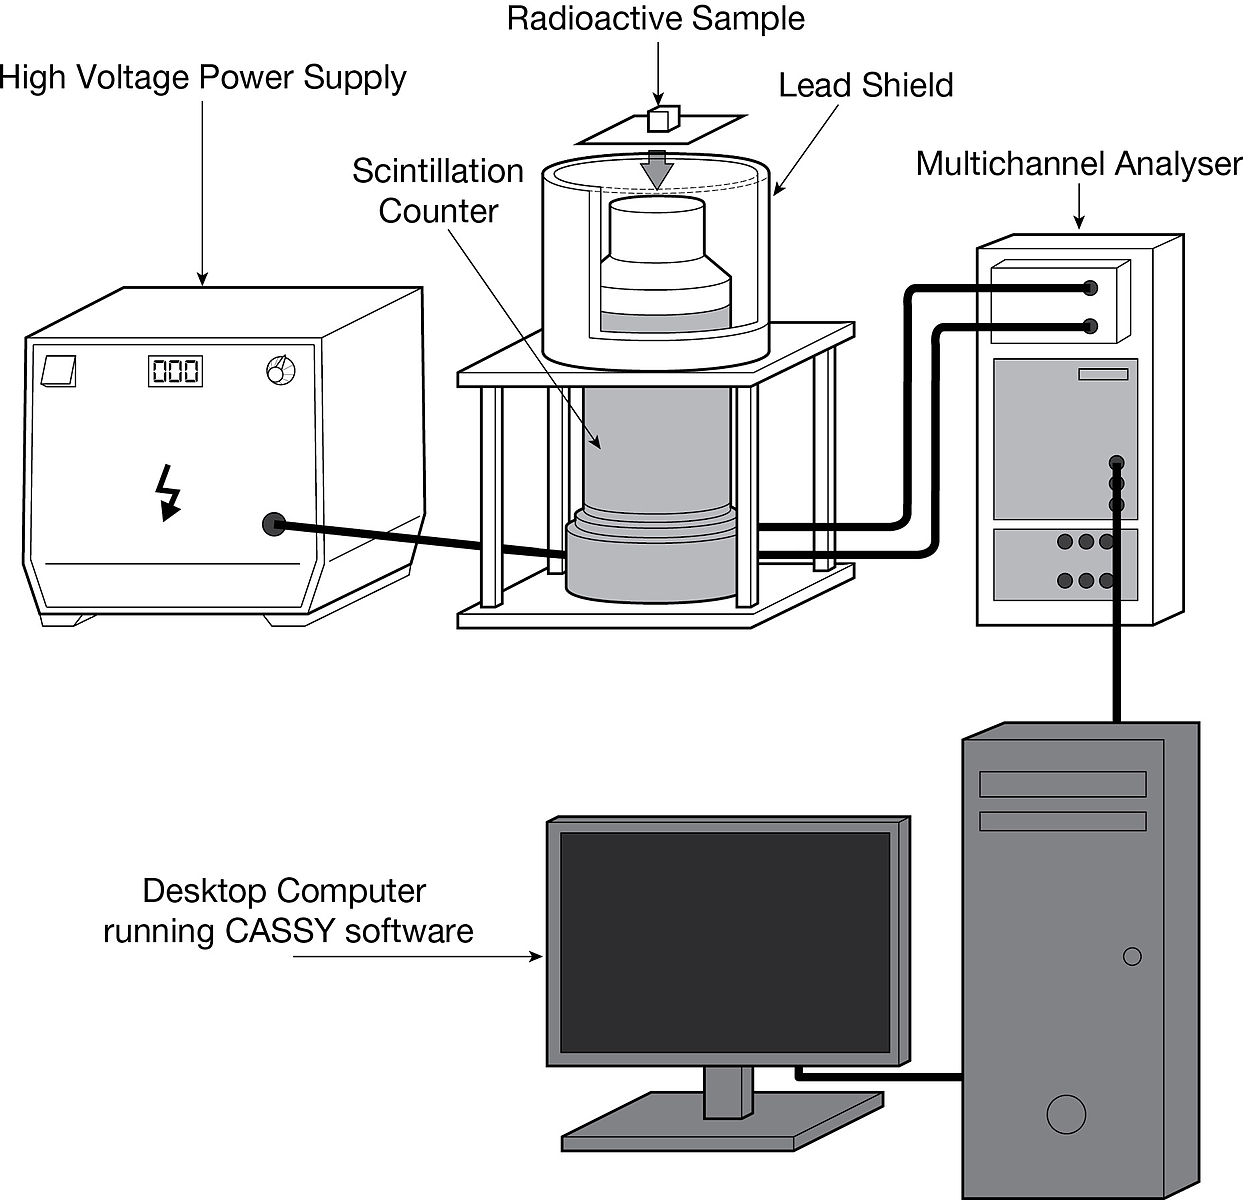
\includegraphics[width=0.6\textwidth]{diagram.jpg}
    \vfill
\end{center}

\pagebreak
\setstretch{1.6}
\paragraph{\textbf{The Objective} of this experiment was to familiarize ourselves with the technique of nuclear spectroscopy, and to explore the effects of using shielding materials in this technique.}

\section{Theoretical Background/ Abstract}
\setstretch{1.8}
Nuclear decay (or radioactivity) is a process that occurs in nuclei of unstable isotopes of typically heavy elements---those with high atomic number. In this process, an energetic proton or neutron will spontaneously decay into a beta particle or an alpha particle respectively, as well as some gamma rays to account for energy conservation. This process is said to be stochastic, making it impossible to predict when a particular atom will decay. Despite this, each isotope has some has some known probability for nuclear decay, so for a large arrangement of atoms, decay rate will be fairly predictable. The time it takes for half the atoms in a given substance to decay is known as its half-life. This value is consistent for all samples of a given isotope, but can vary tremendously across different substances. The shortest recorded half-life is on the scale of $10^{-23}$ seconds (Hydrogen-5 and -7), while the longest is held by Tellurium-128 at $10^{24}$ years, which is much longer than the universe has existed!\\

In this lab, we will examine the nuclear decay processes of Cesium-137, which has a half-life of 30.2 years. This may seem like too long a time for this isotope to be a good experimental subject, but it's actually ideal: The instruments we will use in this lab are sensitive to the decay of individual beta particles. For a 1 mole sample of Cesium-137, containing approximately Avogadro's number of atoms, we can expect to see a large amount of nuclear activity in our minute-scale sampling period. Isotopes with a longer half-life would decay too slowly, and those with short half-lives are to volatile to be studied, as their decay rate exceeds the sampling rate of our instrumentation.\\

When a radioactive isotope decays into its daughter product, it also emits gamma rays with a some regular frequency spectrum. Analyzing this spectrum can be used to identify the composition of the decaying source material. Examining the characteristic energy spectra emitted from a decaying radioactive isotope is known as nuclear spectroscopy.\\

\begin{figure}[H]
    \centering
    \label{graph}
    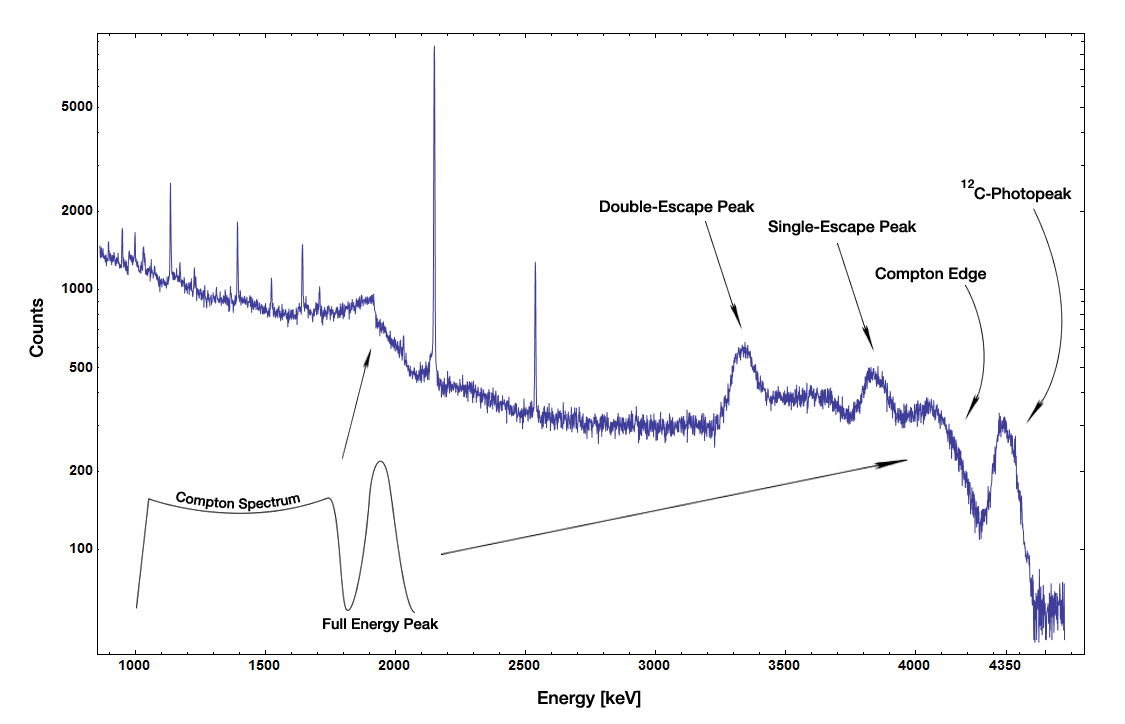
\includegraphics[width=0.6\textwidth]{graph.jpg}
    \caption{The Energy Spectrum of A Radioactive Isotope}
\end{figure}

Beta decay is a process in which the proton of an atom is transformed into a neutron, or vice-versa. This happens inside the atom's nucleus, which the resultant particles and energy soon escape. There are two types of beta decay, $\beta^-$ and $\beta^+$. As you may have guessed, $\beta^-$ decay produces a negatively charged particle (among other things), where $\beta^+$ produces a positively-charged particle, known as a positron.
\begin{equation}
    \label{betaplus}
    p \rightarrow n + \beta^+ + \nu_e
\end{equation}
Where $\beta^+$ is a so-called beta particle: a high-energy, high-speed positron emitted in radioactive decay. The twin decay process, $\beta^-$-decay, is characterized by the following reaction formula:
\begin{equation}
    n \rightarrow p + \beta^- + \bar\nu_e
\end{equation}
$\beta^-$ is again a beta particle, but this time it's an electron instead of a positron. $\bar\nu_e$ is an \textbf{electron anti-neutrino}, the antiparticle of the electron neutrino shown in Equation \ref{betaplus}. It's largely there to make sure that energy is conserved in the decay process. To calculate the energy of a beta particle incident on our detector, we must take into account the energy lost by the ionization and excitation of particles in our detection apparatus. This gives us the following:
\begin{equation}
    \dfrac{{\rm d}E}{{\rm d}x} \propto \dfrac{z^2e^2NZ}{mV^2}
\end{equation}
Where $Z$ is the atomic number of the absorber, $N$ is the atomic density of the absorber, in particles-per-length-cubed, and $V$ is the speed of the radiation. $E, x, e, {\rm and} m$ hold the conventional meanings.
\begin{equation}
    \sigma_{pe} \approx {\rm constant} \dfrac{Z^4}{(h\nu)^3}
\end{equation}

\begin{equation}
    \label{compton}
    E_{\gamma}\prime = \dfrac{1}{1+(E_{\gamma}/mc^2)(1-\cos\phi)}
\end{equation}

\begin{equation}
    I = I_0e^{-\mu x}
\end{equation}

\section{Experimental Procedure}
\setstretch{1.3}
\begin{enumerate}
\item Turn on the amplifier and geiger counter assemblies.
\item Turn on the computer and open the software interface.
\item Ensure that all the connections are made between the geiger counter, the amplifier, and the software interface.
\item Remove the 3 lead bricks from the front of the spectroscopy enclosure, making sure not to lick them in the process.
\item Do not drop them on your feet either.
\item Or your partner's feet.
\item Place a test sample in the measurement enclosure to make sure that your geiger counter is working properly. Take a small spectroscopy measurement as well.
\item Tune the measuring parameters to the settings marked in your lab manual:
Multichannel Measurement, Number of Channels = 512, Measuring Time = 20 s, $\checkmark$ in Negative Pulses box, Gain Slider = X1
\item Turn the voltage on the power supply to 600V.
\item place the Cs-137 inside the spectroscopy enclosure.
\item Return the lead bricks to the spectroscopy enclosure.
\item Run the CASSY software interface and don't forget to save your datums.
\item Place shields of varying composition and thickness in between the sample and the geiger counter.
\item Observe their effect.
\item Do the same for the Americanium.
\end{enumerate}
\setstretch{1.8}
\vfill

\section{Graphs and Tables}
\begin{figure}[H]
    \begin{minipage}{0.49\textwidth}
        \centering
        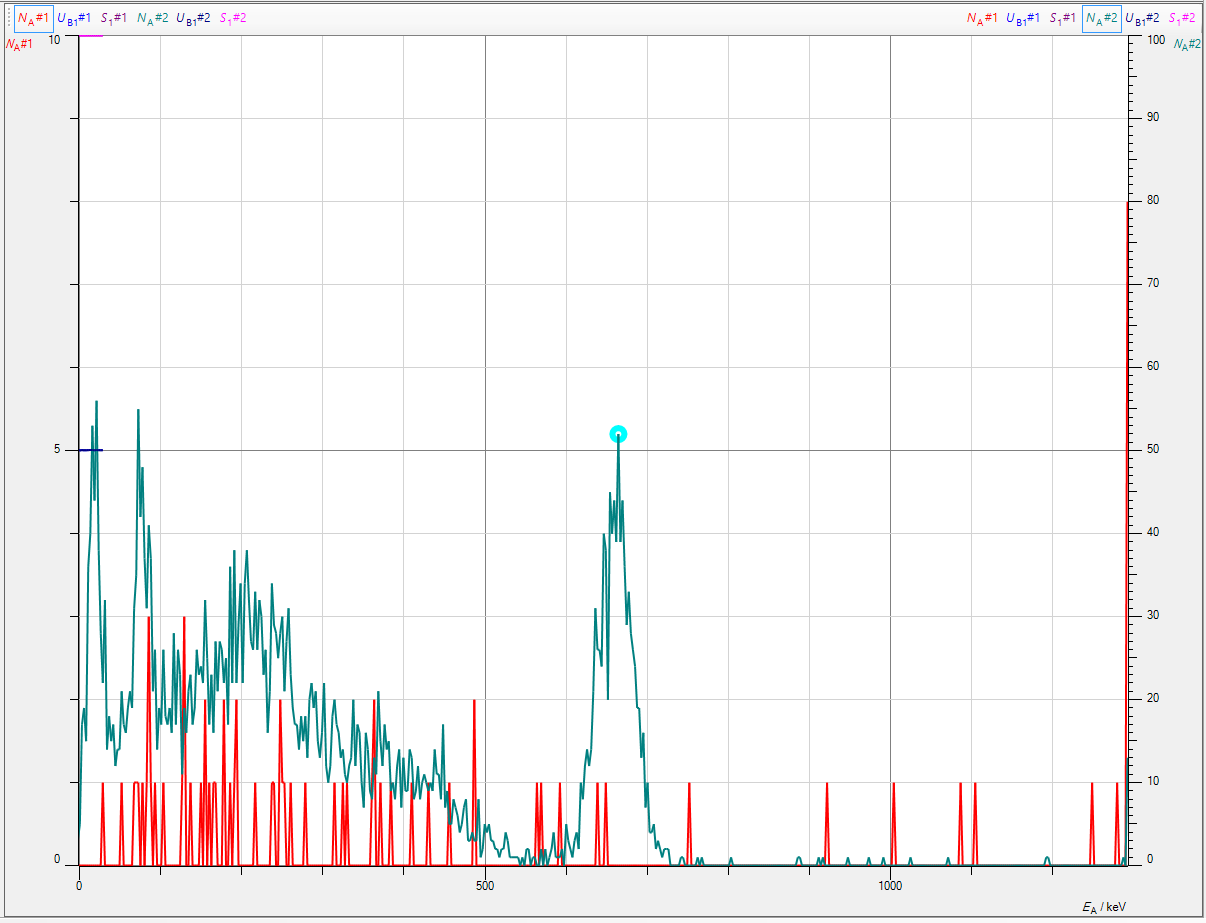
\includegraphics[width=\textwidth]{CSnoise.png}
        \caption{\newline Cs-137 and Background Noise}
    \end{minipage}
    %
    \begin{minipage}{0.49\textwidth}
        \centering
        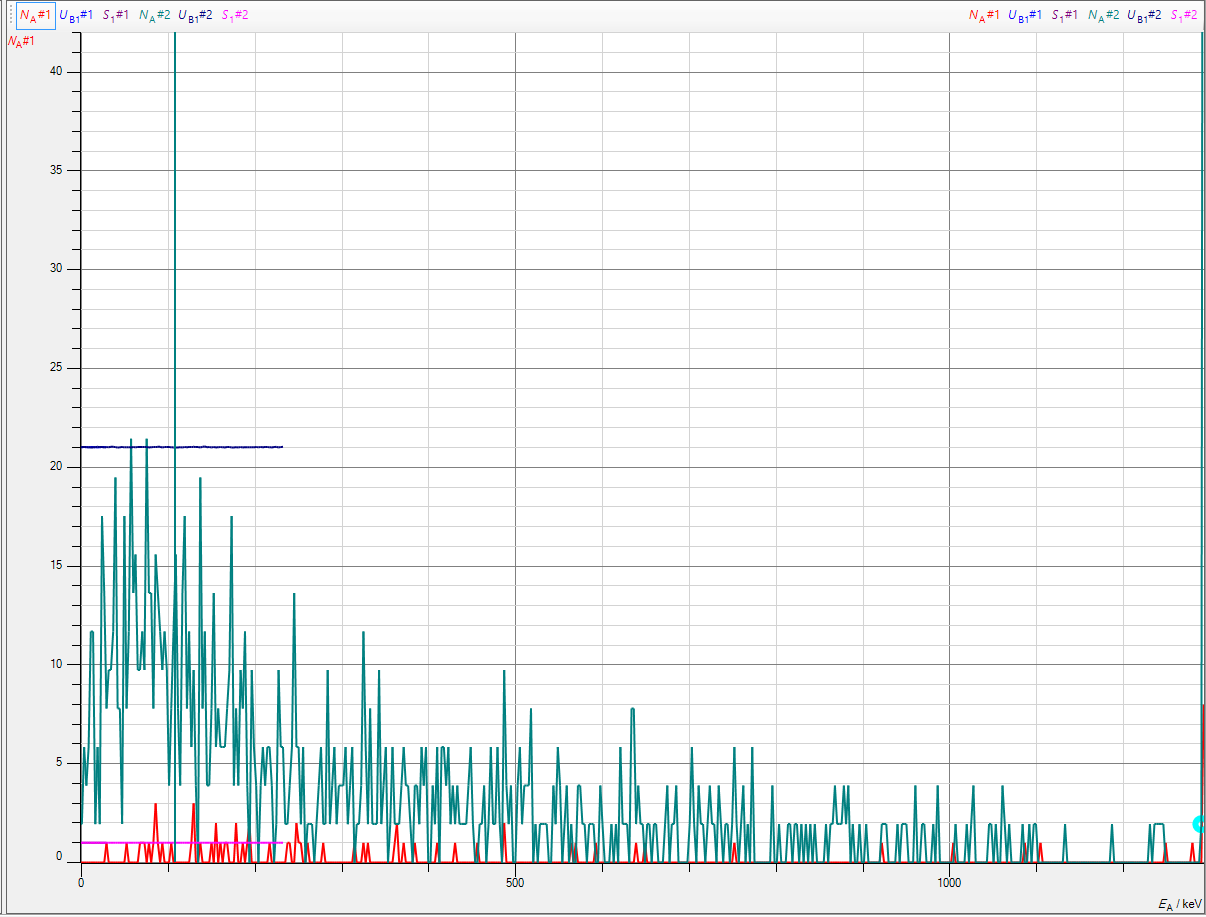
\includegraphics[width=\textwidth]{Sr-90.png}
        \caption{\newline Sr-90 and Background Radiation}
    \end{minipage}
\end{figure}

\begin{table}[h]
\centering
\caption{Energies of Peak Spectra in Two Materials}
\label{my-label}
\begin{tabular}{c|c|c}
Material & bin \#  & Energy (keV)   \\ \hline
Am-241   & 32      & 59.54          \\
Cs-137   & 266     & 661.66
\end{tabular}
\end{table}

\begin{table}[h]
\centering
\caption{Measuring the Effects of Various Shields}
\label{my-label}
\begin{tabular}{l|l|l}
Material & Thickness (mm) $\pm 0.1$mm & N      \\ \hline
None     & 0                          & 10338  \\
Aluminum & 2.1                        & 10345  \\
Aluminum & 3.1                        & 10176  \\
Copper   & 3.0                        & 9495   \\
Lead     & 1.1                        & 9246   \\
Lead     & 2.4                        & 7862   \\
Lead     & 3.4                        & 6849   \\
Lead     & 8.4                        & 4980
\end{tabular}
\end{table}

As can be seen, aluminum seems to had no effect in blocking the radiation of Cesium-137. This is likely due to the fact that its absorption spectrum does not overlap with the emission spectrum of cesium. It is therefore said to be ``transparent" to these energies. I would feel more confident in this assertion if we had been given a greater variety in thickness of aluminum shields, but alas, we were not. Lead, as you can plainly see from the above table as well as the python plot below, has a large effect on the shielding the beta radiation of cesium. It follows that a peak along its absorption spectrum lines up nicely with cesium's characteristic energy emission level. The absorption coefficient that we determined for lead was about $e^{-0.42} \approx 0.6 \mu / {\rm mm^2}$, given by the exponent of the slope of our logarithmic plot (done to use the linear chi-squared fit technique).

\begin{figure}[H]
    \centering
    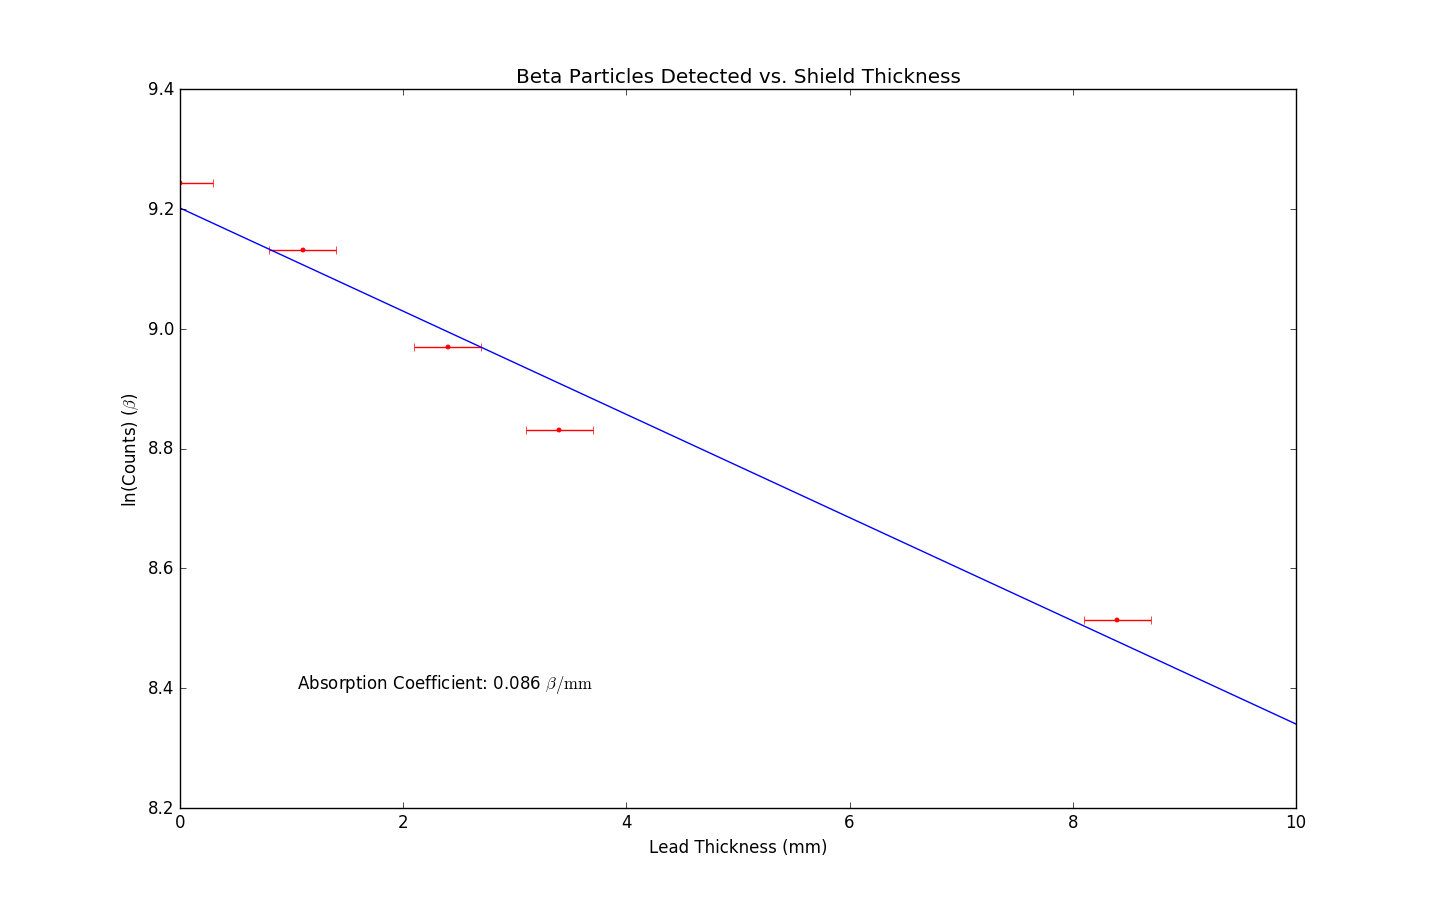
\includegraphics[width=\textwidth]{fitted.png}
    \caption{Calculating the Absorption Coefficient of Lead}
\end{figure}

\section{Questions}

\begin{enumerate}
    \item {\textit{How does the absorption coefficient depend on the mass density of the absorber?}\\
        Given that lead, and very dense material, was a better absorber than copper (which is a less-dense material) is indication that higher mass density positively affects the absorption coefficient of a material. I'd guess, however, that this mass density is not the only factor that influences the absorption coefficient: other metrics, like the arrangement of atoms in a given material, also contribute to its absorption coefficient.
    }
    \item {\textit{How does the absorption coefficient depend on the energy of the gamma ray?}\\
        Higher energy gamma rays have less trouble getting through a material than less energetic rays, which is to say that the energy of a gamma ray in inversely correlated to the absorption coefficient of a shielding material.
    }
\end{enumerate}
\section{Analysis}


$(e^-0.086127929423935143, 9.2016249483377557)$

\end{document}
